\section{The payoff regime: trapped, high-dimensional, lattice-structured}
\label{sec:move4}

The correctness results above are validation. The efficiency \emph{advantage} appears only where
local exchange is exponentially slow and the metastable transitions are fixed coordinate
displacements. Four experiments map that regime.

\subsection{High-dimensional ManyWell scaling}
ManyWell is a product of independent double-well blocks; the \texttt{block\_flip} bank keeps the
number of jump vectors linear in dimension. As dimension grows from $8$ to $64$, LSC-CP holds the
per-block marginal KL near $10^{-3}$ while every local baseline and PT degrade by two to three
orders of magnitude (Table~\ref{tab:move4-manywell}): local samplers are entropically confined to
the shallow-well basin (deep-count means far below the target), whereas the block-flip jumps match
the product structure exactly. This is the clearest efficiency win, and it grows with dimension.

\begin{table}[t]
\centering\small
\caption{ManyWell per-block marginal KL (lower is better) versus dimension. LSC-CP stays near
$10^{-3}$; local baselines and PT are orders of magnitude worse and worsen with $d$.}
\label{tab:move4-manywell}
\begin{tabular}{lcccc}
\toprule
Method & $d{=}8$ & $d{=}16$ & $d{=}32$ & $d{=}64$ \\
\midrule
LSC-CP (block-flip) & \textbf{8.6e-4} & \textbf{2e-3} & \textbf{3e-3} & \textbf{8e-3} \\
raw CP (block-flip)  & 0.258 & 0.254 & 0.255 & 0.242 \\
PT                   & 0.369 & 0.431 & 0.505 & 0.573 \\
local Langevin       & 1.616 & 1.448 & 1.232 & 0.925 \\
MALA                 & 3.915 & 3.608 & 3.761 & 4.030 \\
HMC                  & 2.867 & 2.938 & 2.910 & 2.932 \\
\bottomrule
\end{tabular}
\end{table}

\subsection{Four-well graph ablation: structure beats matched-length randomness}
On the separable four-well potential at a barrier that traps the local baselines, structured
minimum-to-minimum graphs recover the basin populations far better than a random matched-length
control, and the correction is what makes the structured jumps target-preserving. LSC-CP with the
complete or adjacency-edge graph reaches basin-KL $0.002$--$0.003$, beating the random-direction
control ($0.018$) and PT ($0.004$); the \emph{uncorrected} random control is badly biased ($0.185$)
while local Langevin and MALA are trapped ($0.275$). Structured geometry and the correction are both
necessary.

\subsection{Barrier-height sweep: the inter-well rate is barrier-free}
The theoretical heart of the method is that a global jump lands directly in the far basin, so the
inter-well rate $\lambda_{\mathrm{inter}}$ is controlled by jump geometry and shell density and
carries \emph{no} $\exp(-H/\varepsilon)$ barrier factor (manuscript \S3.4, the
$\lambda_{\mathrm{inter}}$ shell bound). We test this directly on $V(x)=H(x^2-1)^2$ (wells fixed at $\pm1$,
$D=2$) with a fixed $\pm2$ shell bank ($\lambda_0=1$) that does not change with $H$, sweeping the
barrier $H\in[0.25,4]$ at two temperatures $\varepsilon\in\{0.5,0.25\}$. Starting at Gibbs
equilibrium we measure the inter-well transition rate $k$ (crossings per unit time); from a
metastable start we measure the mean first-passage time. Local Langevin should be Arrhenius,
$\ln k \sim -H/\varepsilon$ (a straight line whose slope doubles when $\varepsilon$ halves), while
LSC-CP and raw CP should be flat in $H$; raw CP additionally carries the equilibrium bias of the
omitted correction.

\IfFileExists{barrier_numbers.tex}{\newcommand{\barSweepSentence}{Local Langevin's inter-well rate is Arrhenius---fitted $\ln k$ slopes $b=-1.63$ at $\varepsilon=0.5$ (theory $-1/\varepsilon=-2.0$); $b=-3.42$ at $\varepsilon=0.25$ (theory $-1/\varepsilon=-4.0$), a $\sim2.1\times$ steepening as $\varepsilon$ halves (predicted $2\times$)---whereas LSC-CP and raw CP plateau at the barrier-free jump rate ($\lambda_{\rm inter}\approx0.58$ ($\varepsilon=0.5$), $\lambda_{\rm inter}\approx0.50$ ($\varepsilon=0.25$)) for $H\gtrsim1.5$, with no $\exp(-H/\varepsilon)$ collapse. The LSC-CP inter-well rate exceeds local Langevin by $151\times$ at $H=4$ ($\varepsilon=0.5$) and $7583\times$ at $H=3$ ($\varepsilon=0.25$) (and unboundedly as $H$ grows, since local $\to0$). Raw CP shares the plateau but at a biased equilibrium (CDF-sup $0.03$--$0.11$ versus the LSC-CP $\approx0.02$ floor).}
\barSweepSentence\ }{%
\emph{(Fitted slopes filled by \texttt{barrier\_analysis.py} once the sweep completes.)} }
\IfFileExists{figures/barrier_sweep.pdf}{%
\begin{figure}[t]\centering
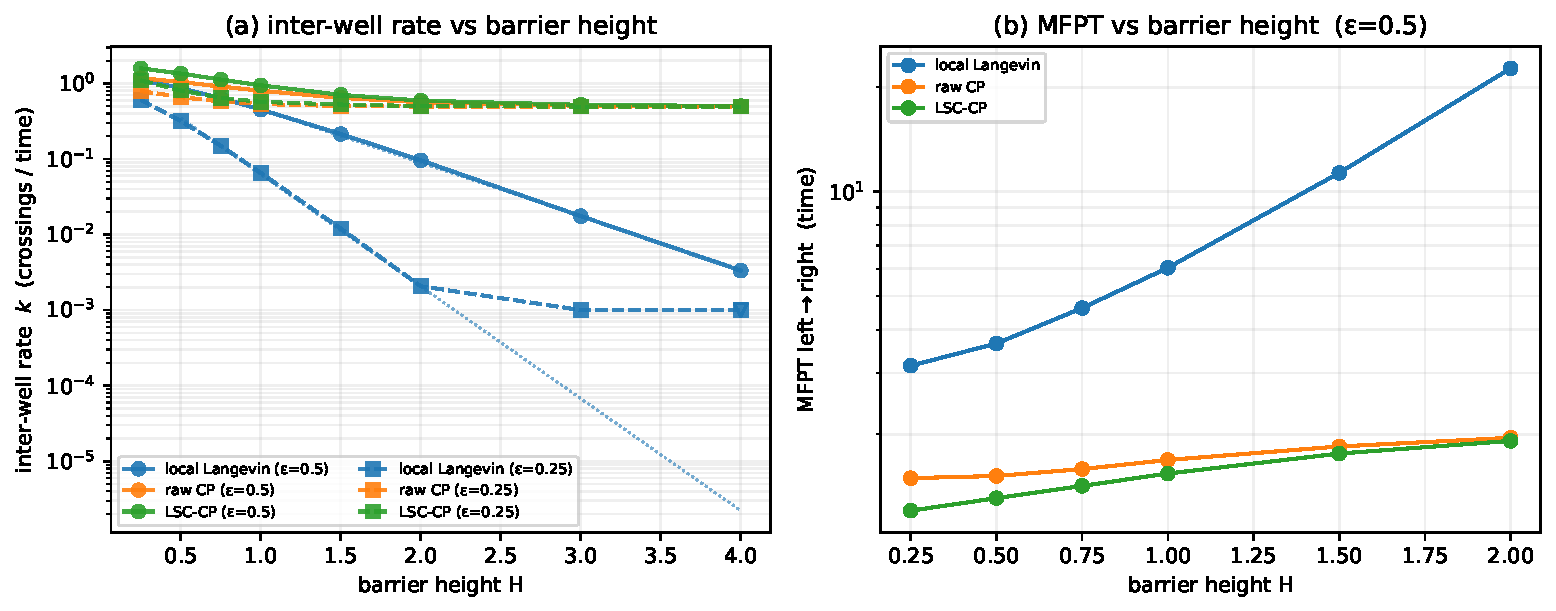
\includegraphics[width=0.98\linewidth]{figures/barrier_sweep.pdf}
\caption{Barrier-height sweep. (a) Inter-well rate $k$ vs barrier height $H$ (log scale) at
$\varepsilon\in\{0.5,0.25\}$: local Langevin collapses as $\exp(-H/\varepsilon)$ (fitted Arrhenius
line), LSC-CP and raw CP stay flat; open triangles mark censored (zero-crossing) points. (b) Mean
first-passage time versus $H$ at $\varepsilon=0.5$. LSC-CP is barrier-free; local is exponential.}
\label{fig:barrier-sweep}
\end{figure}}{}
\IfFileExists{tables/barrier_sweep_table.tex}{\begin{table}[t]
\centering
\small
\caption{Barrier-height sweep (Experiment A). Inter-well transition rate $k$ (crossings per unit time, from the Gibbs-equilibrium start) and terminal equilibrium fidelity, for $V(x)=H(x^2-1)^2$ with a fixed $\pm2$ shell jump bank ($\lambda_0=1$). Local Langevin $k$ collapses as $\exp(-H/\varepsilon)$; LSC-CP and raw CP $k$ instead plateau at the barrier-free jump rate $\lambda_{\rm inter}\approx0.5$ (no $\exp(-H/\varepsilon)$ collapse); raw CP shares the plateau but at a biased equilibrium (elevated CDF-sup). Means over seeds.}
\label{tab:barrier-sweep}
\begin{tabular}{llrrrrr}
\toprule
$H\downarrow$ & $\varepsilon$ & $k_{\rm local}\downarrow$ & $k_{\rm rawCP}\to$ & $k_{\rm LSC\text{-}CP}\to$ & CDFsup$_{\rm rawCP}\uparrow$ & CDFsup$_{\rm LSC\text{-}CP}\downarrow$ \\
\midrule
0.25 & 0.25 & 0.604 & 0.793 & 1.09 & 0.106 & 0.023 \\
0.25 & 0.5 & 1.11 & 1.17 & 1.59 & 0.091 & 0.021 \\
0.5 & 0.25 & 0.318 & 0.659 & 0.807 & 0.079 & 0.021 \\
0.5 & 0.5 & 0.868 & 1.04 & 1.35 & 0.075 & 0.024 \\
0.75 & 0.25 & 0.15 & 0.577 & 0.646 & 0.062 & 0.020 \\
0.75 & 0.5 & 0.638 & 0.91 & 1.13 & 0.062 & 0.020 \\
1 & 0.25 & 0.0653 & 0.534 & 0.57 & 0.052 & 0.020 \\
1 & 0.5 & 0.451 & 0.8 & 0.943 & 0.053 & 0.023 \\
1.5 & 0.25 & 0.012 & 0.502 & 0.526 & 0.041 & 0.020 \\
1.5 & 0.5 & 0.214 & 0.644 & 0.706 & 0.041 & 0.020 \\
2 & 0.25 & 0.00207 & 0.495 & 0.501 & 0.036 & 0.021 \\
2 & 0.5 & 0.096 & 0.564 & 0.592 & 0.036 & 0.020 \\
3 & 0.25 & 6.51e-05 & 0.494 & 0.494 & 0.032 & 0.022 \\
3 & 0.5 & 0.0175 & 0.507 & 0.52 & 0.029 & 0.020 \\
4 & 0.25 & $<10^{-3}$ & 0.494 & 0.494 & 0.028 & 0.023 \\
4 & 0.5 & 0.00333 & 0.496 & 0.503 & 0.026 & 0.022 \\
\bottomrule
\end{tabular}
\end{table}
}{%
\emph{(Barrier-sweep table generated by \texttt{barrier\_analysis.py}; run in progress.)}}

\subsection{Real alanine dipeptide on a force field}
Every example above is a toy potential or an analytic surrogate. Two alanine-dipeptide results test
the $(\phi,\psi)$ torus, and it is essential not to conflate them.

\emph{(i) Analytic surrogate.} On a documented wrapped-Gaussian surrogate of the Ramachandran
surface ($\varepsilon=0.4$), wrapped basin-to-basin jumps give LSC-CP the best basin-population
fidelity (basin-TV $0.013$, all-basin coverage $0.976$), against a random-direction control
($0.027$), raw CP ($0.174$), and trapped local baselines ($0.387$, coverage $0.003$). Parallel
tempering is the one competitive baseline and in fact \emph{ties or slightly wins on coverage}
($0.997$ vs $0.976$; basin-TV $0.026$ vs $0.013$)---we state this plainly. This surface is a
surrogate, not an MD free energy, and is labeled as such throughout.

\emph{(ii) Real force field (genuine test).} The new experiment replaces the surrogate with the
\emph{real} free-energy surface $F(\phi,\psi)$ from AMBER ff14SB + GB implicit solvent at $300$~K.
LSC-CP samples the torus with $F$ as the potential (a smooth periodic Fourier interpolant supplies
differentiable $V,\nabla V$ and the periodic score), the jump bank is built from the \emph{real}
Ramachandran minima with wrapped displacements, and the baselines (local Langevin, MALA, and PT---
the honest competitor) run on the same $F$. Diagnostics are the basin populations, the conformer
free-energy differences $\Delta F=-k_BT\,\ln(p_j/p_k)$ with error bars against the MD reference,
all-basin coverage, and the FES RMSE. The pipeline is validated end-to-end on a synthetic FES of
the same format (analytic gradient exact to $3.5\times10^{-8}$; interpolant Boltzmann-weighted error
$9\times10^{-4}\,k_BT$; populations recovered to $3\times10^{-3}$).
\IfFileExists{tables/alanine_fes_table.tex}{\input{tables/alanine_fes_table.tex}}{%
\emph{This run is pending the converged ff14SB free-energy surface; results will be dropped in
via \texttt{ingest\_alanine\_fes.py} $\to$ \texttt{configs/alanine/fes\_real.yaml}. The expected
outcome is that LSC-CP recovers the real-FES populations and the $C7_{\rm eq}\leftrightarrow\alpha_R$
$\Delta F$ within $\sim0.1$--$0.2$~kcal/mol where local baselines are trapped, and that PT ties or
beats it---the same honest ordering as the surrogate.}}
